\documentclass{ximera}

\input{preamble.tex}

\author{Gregory Hartman \and Matthew Carr}
\license{Creative Commons 3.0 By-NC}
\acknowledgement{https://github.com/APEXCalculus}

\begin{document}
\begin{exercise}

\outcome{Explain the relationship between one-sided and two-sided limits.}

\tag{limit} 

\noindent\begin{minipage}[t]{.5\linewidth}
\begin{center}
 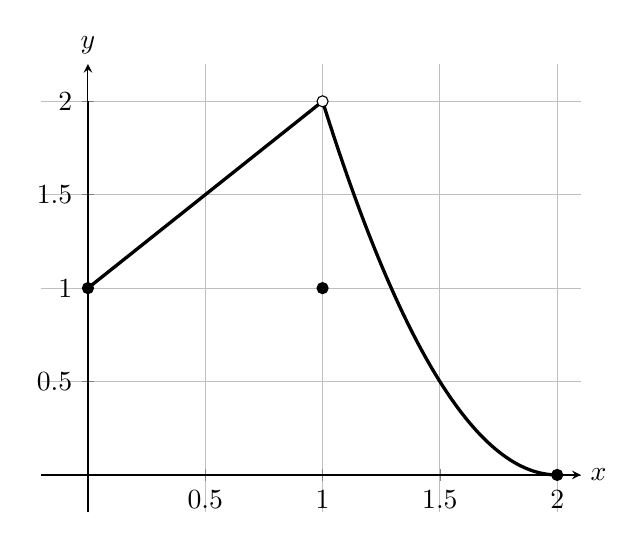
\begin{tikzpicture}
	\begin{axis}
	[ymin=-0.2,ymax=2.2, axis lines=center,xlabel=$x$,ylabel=$y$,every axis y 
	label/.style={at=(current axis.above origin),anchor=south},every axis x label/.style={at=(current axis.right of origin),anchor=west},
	domain=-1:2,
	ytick={0.5,1,1.5,2},
	yticklabels={$0.5$,$1$,$1.5$,$2$},
	xtick={0.5,1.0,1.5,2},
	xticklabels={$0.5$,$1$,$1.5$,$2$},
	ymajorgrids=true,
	grid = major
	]
	\addplot[domain=0:2,very thick,smooth,samples=600]
	{(!(\x>1))*(\x+1)+(\x>1)*(!(\x>2))*(2*(\x-2)^2};
	\addplot[domain=-0.2:2.1, smooth, very thin, samples=100,color=black]
	{0};
	\draw[very thin,color=black] (axis cs:0,-0.2) -- (axis cs:0,2);
	\draw[fill=black] (axis cs:0,1) circle [radius=2pt];
	\draw[fill=black] (axis cs:2,0) circle [radius=2pt];
	\draw[fill=black] (axis cs:1,1) circle [radius=2pt];
	\draw[fill=white] (axis cs:1,2) circle [radius=2pt];
	\end{axis}
       \end{tikzpicture}
    \end{center}
\end{minipage}
       
\noindent\begin{minipage}[t]{.5\linewidth}
\begin{enumerate}
\item		$\lim_{x\to 1^-} f\p{x}$
\item		$\lim_{x\to 1^+} f\p{x}$
\item		$\lim_{x\to 1} f\p{x}$
\end{enumerate}
\end{minipage}
\noindent\begin{minipage}[t]{.5\linewidth}
\begin{enumerate}\addtocounter{enumii}{3}
\item		$f\p{1}$
\item		$\lim_{x\to 0^-} f\p{x}$
\item		$\lim_{x\to 0^+} f\p{x}$
\end{enumerate}
\end{minipage}

{\begin{enumerate}
\item		2
\item		2
\item		2
\item		1
\item	 	As $f$ is not defined for $x<0$, this limit is not defined.
\item		1
\end{enumerate}}

\end{exercise}
\end{document}